\documentclass{article}
\usepackage{graphicx}
\usepackage{algorithmic}
\title{relabel algorithm and its support for parametric computing}
\author{zhaofeng-shu33}
\begin{document}
\maketitle
In the implementation of Preflow algrithms, we differentiate
two types of \textbf{push}. One is normal push, that is,
$f_{uv} < c_{uv}$ and $x_u >0$, $u$ can push some stored flow
to $v$. The other is \textbf{push back}, that is,
$f_{vu} >0$ and $x_u >0$ and $u$ can push some stored flow back to $v$.

\begin{figure}[!ht]
\centering
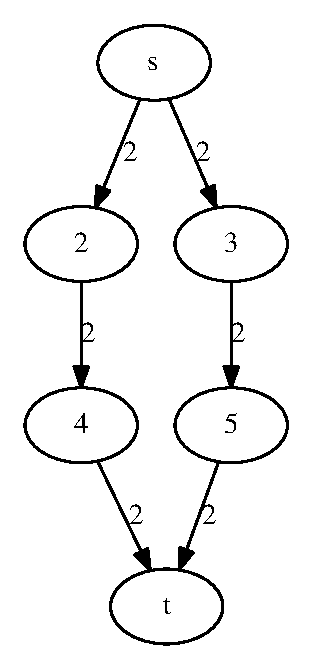
\includegraphics[width=6cm]{fig/size.eps}
\caption{minimum cut is not unique}\label{fig:mc}
\end{figure}

In figure \ref{fig:mc}, our algrithm (Preflow\_Relabel) will produce the minimum cut whose source side is of maximal size.

\begin{figure}[!ht]
\centering
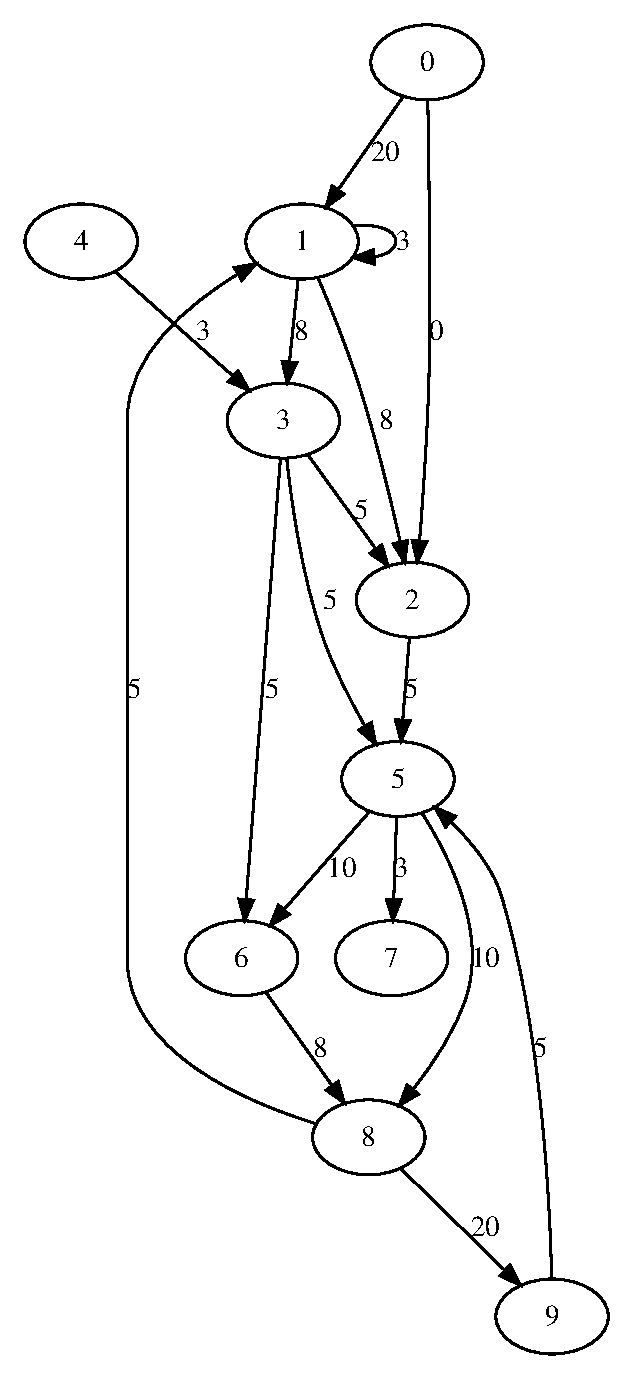
\includegraphics[width=6cm]{fig/test.eps}
\caption{minimum cut is not unique}\label{fig:ex}
\end{figure}

Figure \ref{fig:ex} is the official example of lemon library when testing Preflow algorithm, notice that Node 0 and Node 7 will never be reached. Therefore, their belonging in min-cut seems arbitrary. 

In the Relabel algorithm, we assume $d(S) $ is the maximal label in the graph, when $c(s,v)$ increases, we need to reinit the preflow algorithm. Only node with $d(v) <= d(S) + 1$ can be pushed to make node $v$ active. This is the valid labeling constraint. For the target node, there is no constraint. We summarize the reinit function as follows(We assume the capacity is modified limited at edge set $\{(v,t)\in E\}\cup \{(s,u)\in E\}$)
\begin{algorithmic}[1]
\REQUIRE graph $G(V,E)$, valid label $d(v)$, excess function $e(v)$ and modified capacity map $c(u,v)$ and flow function $f(u,v)$.
\ENSURE a valid preflow $f'(u,v)$ and excess function $e'(v)$.
\FOR{node $v$ such that $(v,t)\in E$}
\IF{$f(v,t)>c(v,t)$}
\STATE $e(v) = f(v,t)-c(v,t)$
\STATE $f(v,t)=c(v,t)$
\ENDIF
\ENDFOR
\FOR{node $u$ such that $(s,u)\in E$}
\IF{$f(s,u)<c(s,u)$ and $u \neq t$ and $d(u)\leq 1+d(s)$}
\STATE $e(v) = c(s,u)-f(s,u)$
\STATE $f(s,u)=c(s,u)$
\ENDIF
\ENDFOR
\end{algorithmic}
We use \texttt{speed\_test.cpp} to test the speed of our algorithm. The graph is controled by two parameters,
\texttt{layer\_size} and \texttt{layer\_num}.
\begin{figure}[!ht]
\centering
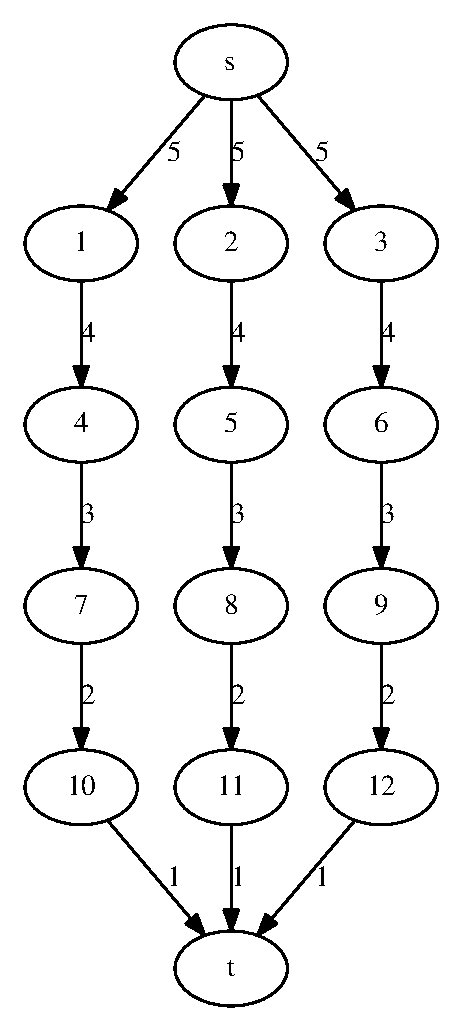
\includegraphics[width=6cm]{fig/normal.eps}
\caption{scalable graph with \texttt{layer\_size} = 3, \texttt{layer\_num} = 4}\label{fig:normal}
\end{figure}
Fig \ref{fig:normal} shows a normal run by invoking the program \texttt{speed\_test}. The parameters can be changed by specifying \texttt{--layer\_size 10}, \texttt{--layer\_num 4} etc.
\begin{figure}[!ht]
\centering
\includegraphics[width=6cm]{fig/reverted.eps}
\caption{scalable reverted graph with \texttt{layer\_size} = 3, \texttt{layer\_num} = 4}\label{fig:reverted}
\end{figure}
Fig \ref{fig:reverted} shows a parametric run by invoking the program \texttt{speed\_test} with \texttt{--parametric}.


\end{document}
